\section{Background}

In the past few decades, many great research contributions and effective decision tools have been implemented to the topic of collision avoidance in air traffic control. Autoresolver, a well-known physics model-based approach, can efficiently generate a series of conflict-free trajectories by employing an iterative method to satisfy all conflict resolution conditions \citep{farley2007fast}. In response to our research focus, the specified sector with multiple intersections and emerging points, National Aeronautics and Space Administration (NASA) has introduced a centralized scheme, known as Traffic Mangement Advisor (TMA) to design such no-conflict time slots and then make sure to maintain seperation distance \citep{erzberger2014design}. In recent years, Artificial intelligence (AI)    technology has been widely used in air traffic management, especially under uncertain decision-making environments which requires highly precise and fast-time simulators to make interaction with the agent. In this way, we employed Bluesky \citep{hoekstra2016bluesky} as our validation framework which was designed by TU Delft and has been extensively applied to relistic and real-time air traffic scenarios.

Multi-agent techniques has seen great success in solving issues related with conflict seolutions and collision avoidance. In early study \citep{wollkind2004automated}, an aircraft was regarded as an agent and negotiation skills were emphasized to resolve appeared conflict warnings. However, in recent works, such communication techniques aren't generally imposed and naturally agents are free to learn the ability through continuous training \citep{brittain2020deep}. Besides, some decentralized algorithms such as multi-agent Monte Carlo Tree Search (MCTS) \citep{yang2020scalable} and Markov Decision Process (MDP) \citep{bertram2020distributed} are formulated to predefine loss of separation (LOS). The LOS situation is introduced from aircraft safety spearation, as shown in Figure \ref{fig:los}. Due to the characteristcs of decentralized framework, these algorithms present priorer performance and faster convergence rate to those with the centralized scheme.

\begin{figure}[H]
    \centering
    \subfigure[Aircraft Safety Separation]{
        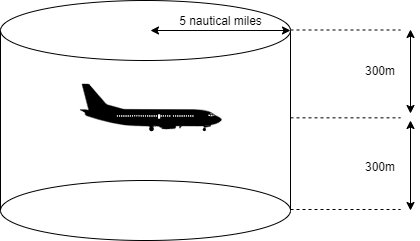
\includegraphics[width=0.365\columnwidth]{images/space.png}
    }
    % \subfigure[$(\epsilon=0.6, T=750)$]{
    %     \includegraphics[width=0.46\columnwidth]{pic/convergence_4-16_n10_ep0.6_T750.png}
    % }
    \subfigure[An Example of LOS]{
        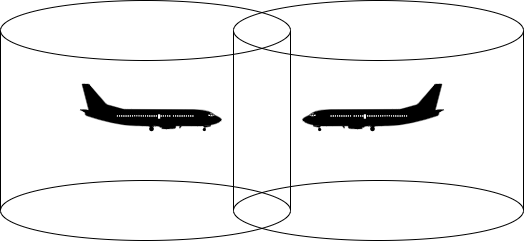
\includegraphics[width=0.46\columnwidth]{images/los.png}
    }
    \caption{The Concept of Aircraft Safety Separation and Loss of Separation}
    \label{fig:los}
\end{figure}

The worst and serious case of LOS could be mid-air collision, and at low altitude, cross-level actions to avoid collision is not commonly applicable, as shown in Figure \ref{fig:collision_level_change}. AI agents such as Alpha Go have shown tremendous advantages in imitating and learning sophisticated human behaviors and even defeated human in some highly dynamic and uncertain competition games through reinforcement learning \citep{mnih2015human}. First related work in aircraft collision avoidance can be traced to \citep{brittain2018autonomous}, where conflicts and delay mitigation are simultaneously emphasized. Then, \cite{pham2019machine} introduces randomness and scenarios analysis to the formulation of the aircraft' maneuvor. However, these approaches fail to consider speed as a vector and the sector structure with multiple emerging points. With this regard, we dedicated to further improve the existing implementation by considering more complex and practical scenarios.

\begin{figure}[H]
    \centering
    \subfigure[Aircraft Safety Separation]{
        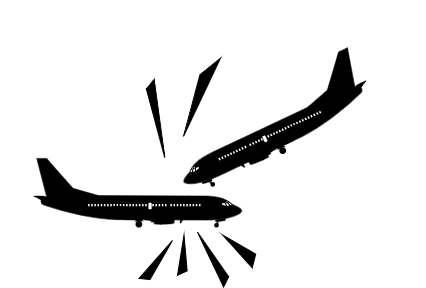
\includegraphics[width=0.35\columnwidth]{images/Mid-air_Collision.png}
    }
    % \subfigure[$(\epsilon=0.6, T=750)$]{
    %     \includegraphics[width=0.46\columnwidth]{pic/convergence_4-16_n10_ep0.6_T750.png}
    % }
    \subfigure[An Example of LOS]{
        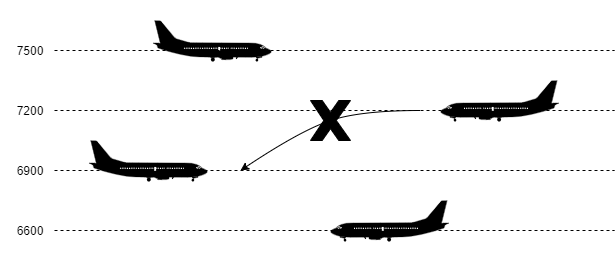
\includegraphics[width=0.46\columnwidth]{images/change_height.png}
    }
    \caption{Mid-air Collision and Flight Level Change Constraint}
    \label{fig:collision_level_change}
\end{figure}

In this work, a distributed deep multi-agent reinforcement learning framework (D2MARL) is proposed to tackle mid-air collision avoidance problems in the sector with multiple intersections and emerging points. 